% Chapter 2: Theory
\section{树状度量空间索引理论基础}

\subsection{树状索引概述}

\subsubsection{基于Pivot Table的索引回顾}

在Assignment 2中,我们实现了Pivot Table索引。Pivot Table通过预计算数据到支撑点(Pivot)的距离,利用三角不等式进行剪枝。其基本原理如下:

对于查询对象$q$、数据对象$x$和支撑点$p$,由三角不等式可得:
\begin{equation}
    |d(q,p) - d(x,p)| \leq d(q,x) \leq d(q,p) + d(x,p)
\end{equation}

因此,如果$|d(q,p) - d(x,p)| > r$,则$d(q,x) > r$,可以排除$x$。

Pivot Table的局限性包括:
\begin{itemize}
    \item 每次查询需要计算到所有pivot的距离
    \item 只能利用全局的pivot信息,不能根据数据分布进行层次化剪枝
    \item 空间开销大,需要存储所有数据到所有pivot的距离
\end{itemize}

\subsubsection{树状索引的基本思想}

树状索引通过递归划分数据集,构建层次化的索引结构。其优势包括:

\begin{itemize}
    \item \textbf{层次化剪枝}:通过树的层次结构,可以提前排除整个子树
    \item \textbf{局部优化}:每个节点可以根据子树的数据分布选择pivot
    \item \textbf{距离计算少}:只计算到访问路径上节点的pivot的距离
    \item \textbf{可扩展性好}:适合大规模数据集
\end{itemize}

\subsubsection{数据划分方式分类}

根据划分方式,树状索引主要分为两类:

\begin{enumerate}
    \item \textbf{超平面划分(Hyperplane Partitioning)}:代表为GH树,使用两个支撑点定义超平面
    \item \textbf{球形划分(Ball Partitioning)}:代表为VP树,使用一个支撑点定义球形边界
\end{enumerate}

图\ref{fig:partition-types}展示了两种划分方式的几何直观。

\begin{figure}[htbp]
    \centering
    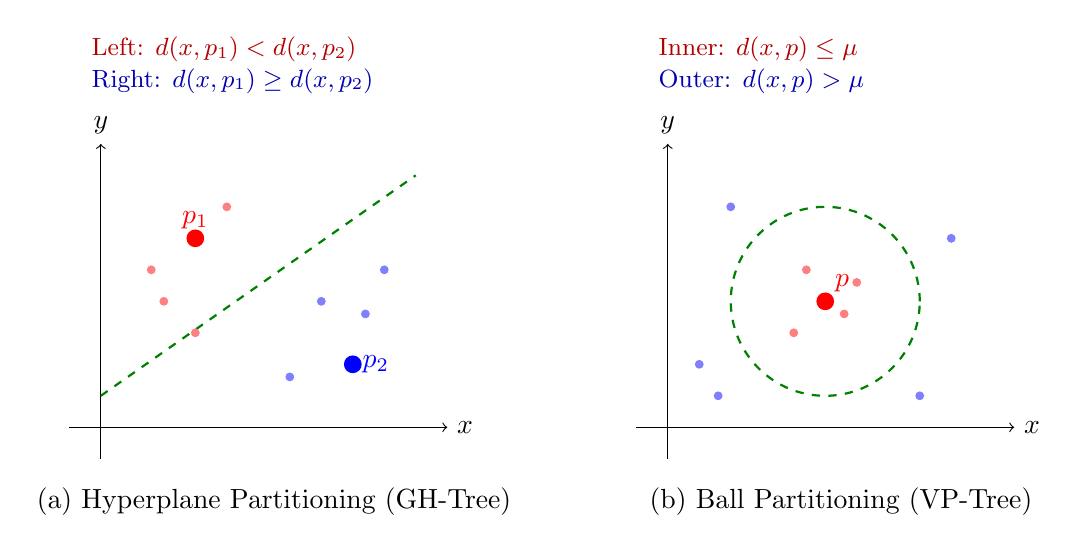
\begin{tikzpicture}[scale=0.8]
        % Hyperplane Partitioning
        \begin{scope}[xshift=0cm]
            \draw[->] (-0.5,0) -- (5.5,0) node[right] {$x$};
            \draw[->] (0,-0.5) -- (0,4.5) node[above] {$y$};

            % Pivot points
            \fill[red] (1.5,3) circle (4pt) node[above] {$p_1$};
            \fill[blue] (4,1) circle (4pt) node[right] {$p_2$};

            % Hyperplane (perpendicular bisector)
            \draw[thick,dashed,green!50!black] (0,0.5) -- (5,4);

            % Data points
            \foreach \x/\y in {1/2, 1.5/1.5, 2/3.5, 0.8/2.5} {
                \fill[red!50] (\x,\y) circle (2pt);
            }
            \foreach \x/\y in {3.5/2, 4.5/2.5, 3/0.8, 4.2/1.8} {
                \fill[blue!50] (\x,\y) circle (2pt);
            }

            \node[anchor=west, red!70!black] at (-0.3,6.0) {\small Left: $d(x,p_1) < d(x,p_2)$};
            \node[anchor=west, blue!70!black] at (-0.3,5.5) {\small Right: $d(x,p_1) \geq d(x,p_2)$};
            \node[below] at (2.75,-0.8) {(a) Hyperplane Partitioning (GH-Tree)};
        \end{scope}

        % Ball Partitioning
        \begin{scope}[xshift=9cm]
            \draw[->] (-0.5,0) -- (5.5,0) node[right] {$x$};
            \draw[->] (0,-0.5) -- (0,4.5) node[above] {$y$};

            % Pivot point
            \fill[red] (2.5,2) circle (4pt) node[above right] {$p$};

            % Ball boundary
            \draw[thick,dashed,green!50!black] (2.5,2) circle (1.5);

            % Inner data points
            \foreach \x/\y in {2.2/2.5, 2.8/1.8, 2/1.5, 3/2.3} {
                \fill[red!50] (\x,\y) circle (2pt);
            }
            % Outer data points
            \foreach \x/\y in {0.5/1, 4.5/3, 1/3.5, 4/0.5, 0.8/0.5} {
                \fill[blue!50] (\x,\y) circle (2pt);
            }

            \node[anchor=west, red!70!black] at (-0.3,6.0) {\small Inner: $d(x,p) \leq \mu$};
            \node[anchor=west, blue!70!black] at (-0.3,5.5) {\small Outer: $d(x,p) > \mu$};
            \node[below] at (2.75,-0.8) {(b) Ball Partitioning (VP-Tree)};
        \end{scope}
    \end{tikzpicture}
    \caption{两种数据划分方式的几何直观}
    \label{fig:partition-types}
\end{figure}

\subsection{GH树(Generalized Hyperplane Tree)}

\subsubsection{基本思想:超平面划分}

GH树使用\textbf{广义超平面}来划分度量空间。给定两个支撑点$p_1$和$p_2$,定义广义超平面为:
\begin{equation}
    H(p_1, p_2) = \{x \in M \mid d(x, p_1) = d(x, p_2)\}
\end{equation}

这个超平面将空间划分为两个区域:
\begin{itemize}
    \item \textbf{左区域}:$L = \{x \in M \mid d(x, p_1) < d(x, p_2)\}$
    \item \textbf{右区域}:$R = \{x \in M \mid d(x, p_1) \geq d(x, p_2)\}$
\end{itemize}

在欧几里得空间中,满足$d(x, p_1) = d(x, p_2)$的点集形成垂直平分线/面。在一般度量空间中,这个集合可能不是平面,故称"广义"超平面。

\subsubsection{数据结构设计}

GH树的节点结构如下:

\textbf{内部节点}包含:
\begin{itemize}
    \item 两个支撑点$p_1$和$p_2$
    \item 左子树指针(离$p_1$更近的数据)
    \item 右子树指针(离$p_2$更近的数据)
    \item 节点深度
\end{itemize}

\textbf{叶子节点}包含:
\begin{itemize}
    \item 数据对象列表
    \item 节点深度
\end{itemize}

\subsubsection{批建算法原理}

GH树的批建算法采用递归方式,如算法\ref{alg:gh-build}所示。

\begin{algorithm}[htbp]
    \caption{GH树批建算法}
    \label{alg:gh-build}
    \begin{algorithmic}[1]
        \REQUIRE 数据集$S$,当前深度$depth$
        \ENSURE GH树节点
        \IF{$|S| \leq maxLeafSize$ \AND $depth \geq minTreeHeight$}
            \RETURN LeafNode($S$, $depth$)
        \ENDIF
        \STATE $(p_1, p_2) \leftarrow$ SelectTwoPivots($S$)
        \STATE $S_{left} \leftarrow \{x \in S \mid d(x, p_1) < d(x, p_2)\}$
        \STATE $S_{right} \leftarrow \{x \in S \mid d(x, p_1) \geq d(x, p_2)\}$
        \STATE $leftChild \leftarrow$ BuildGHTree($S_{left}$, $depth + 1$)
        \STATE $rightChild \leftarrow$ BuildGHTree($S_{right}$, $depth + 1$)
        \RETURN GHInternalNode($p_1$, $p_2$, $leftChild$, $rightChild$, $depth$)
    \end{algorithmic}
\end{algorithm}

\subsubsection{范围查询算法原理}

GH树的剪枝规则是其查询效率的关键。设查询对象为$q$,查询半径为$r$,$d_1 = d(q, p_1)$,$d_2 = d(q, p_2)$。

\textbf{剪枝规则1}(排除左子树):
如果$d_1 - d_2 > 2r$,则可以排除左子树。

\textbf{证明}:左子树中任意数据点$x$满足$d(x, p_1) < d(x, p_2)$。
由三角不等式:
\begin{align}
    d(q, x) &\geq d(q, p_1) - d(x, p_1) = d_1 - d(x, p_1) \\
    d(q, x) &\geq d(x, p_2) - d(q, p_2) = d(x, p_2) - d_2
\end{align}
两式相加:$2d(q,x) \geq d_1 - d(x,p_1) + d(x,p_2) - d_2 > d_1 - d_2$

若$d_1 - d_2 > 2r$,则$d(q,x) > r$,可排除。

\textbf{剪枝规则2}(排除右子树):
如果$d_2 - d_1 > 2r$,则可以排除右子树。

范围查询算法如算法\ref{alg:gh-range}所示。

\begin{algorithm}[htbp]
    \caption{GH树范围查询算法}
    \label{alg:gh-range}
    \begin{algorithmic}[1]
        \REQUIRE 查询对象$q$,查询半径$r$,当前节点$node$
        \ENSURE 满足条件的数据对象列表
        \IF{$node$ is LeafNode}
            \STATE $result \leftarrow \emptyset$
            \FOR{each $x$ in $node.data$}
                \IF{$d(q, x) \leq r$}
                    \STATE add $x$ to $result$
                \ENDIF
            \ENDFOR
            \RETURN $result$
        \ENDIF
        \STATE $result \leftarrow \emptyset$
        \STATE $d_1 \leftarrow d(q, node.p_1)$
        \STATE $d_2 \leftarrow d(q, node.p_2)$
        \IF{NOT $(d_1 - d_2 > 2r)$}
            \STATE $result$.addAll(GHRangeQuery($q$, $r$, $node.leftChild$))
        \ENDIF
        \IF{NOT $(d_2 - d_1 > 2r)$}
            \STATE $result$.addAll(GHRangeQuery($q$, $r$, $node.rightChild$))
        \ENDIF
        \RETURN $result$
    \end{algorithmic}
\end{algorithm}

\subsection{VP树(Vantage Point Tree)}

\subsubsection{基本思想:球形划分}

VP树使用\textbf{球形区域}来划分度量空间。给定一个支撑点(Vantage Point)$p$和划分半径$\mu$,空间被划分为:
\begin{itemize}
    \item \textbf{内球}:$B_{inner} = \{x \in M \mid d(x, p) \leq \mu\}$
    \item \textbf{外球}:$B_{outer} = \{x \in M \mid d(x, p) > \mu\}$
\end{itemize}

通常$\mu$取所有数据到$p$距离的中位数,以保证划分平衡。

\subsubsection{数据结构设计}

VP树的节点结构与GH树类似,但有重要区别:

\textbf{内部节点}包含:
\begin{itemize}
    \item 一个支撑点$p$
    \item 划分中位数$\mu$
    \item 内球子树(距离范围$[L_{inner}, U_{inner}]$)
    \item 外球子树(距离范围$[L_{outer}, U_{outer}]$)
    \item 节点深度
\end{itemize}

关键信息是每个子树的\textbf{距离范围}$[L, U]$,表示该子树中数据到pivot的距离的最小值和最大值。

\subsubsection{批建算法原理}

VP树的批建算法如算法\ref{alg:vp-build}所示。

\begin{algorithm}[htbp]
    \caption{VP树批建算法}
    \label{alg:vp-build}
    \begin{algorithmic}[1]
        \REQUIRE 数据集$S$,当前深度$depth$
        \ENSURE VP树节点
        \IF{$|S| \leq maxLeafSize$ \AND $depth \geq minTreeHeight$}
            \RETURN LeafNode($S$, $depth$)
        \ENDIF
        \STATE $p \leftarrow$ SelectVantagePoint($S$)
        \STATE $distances \leftarrow \{(x, d(x, p)) \mid x \in S, x \neq p\}$
        \STATE Sort $distances$ by distance value
        \STATE $mid \leftarrow |distances| / 2$
        \STATE $S_{inner} \leftarrow distances[0:mid]$
        \STATE $S_{outer} \leftarrow distances[mid:end]$
        \STATE $range_{inner} \leftarrow [\min(S_{inner}.distances), \max(S_{inner}.distances)]$
        \STATE $range_{outer} \leftarrow [\min(S_{outer}.distances), \max(S_{outer}.distances)]$
        \STATE $innerChild \leftarrow$ BuildVPTree($S_{inner}$, $depth + 1$)
        \STATE $outerChild \leftarrow$ BuildVPTree($S_{outer}$, $depth + 1$)
        \RETURN VPInternalNode($p$, $[innerChild, outerChild]$, $[range_{inner}, range_{outer}]$, $depth$)
    \end{algorithmic}
\end{algorithm}

\subsubsection{范围查询算法原理}

VP树的剪枝基于距离范围信息。设查询对象为$q$,查询半径为$r$,$d_q = d(q, p)$,子树$i$的距离范围为$[L_i, U_i]$。

\textbf{剪枝规则1}(内侧剪枝):
如果$d_q + r < L_i$,则可以排除子树$i$。

\textbf{几何解释}:查询球的最远点到$p$的距离为$d_q + r$,如果小于子树中最近点的距离$L_i$,则不相交。

\textbf{剪枝规则2}(外侧剪枝):
如果$d_q - r > U_i$,则可以排除子树$i$。

\textbf{几何解释}:查询球的最近点到$p$的距离为$d_q - r$,如果大于子树中最远点的距离$U_i$,则不相交。

图\ref{fig:vp-pruning}展示了VP树的剪枝规则。

\begin{figure}[htbp]
    \centering
    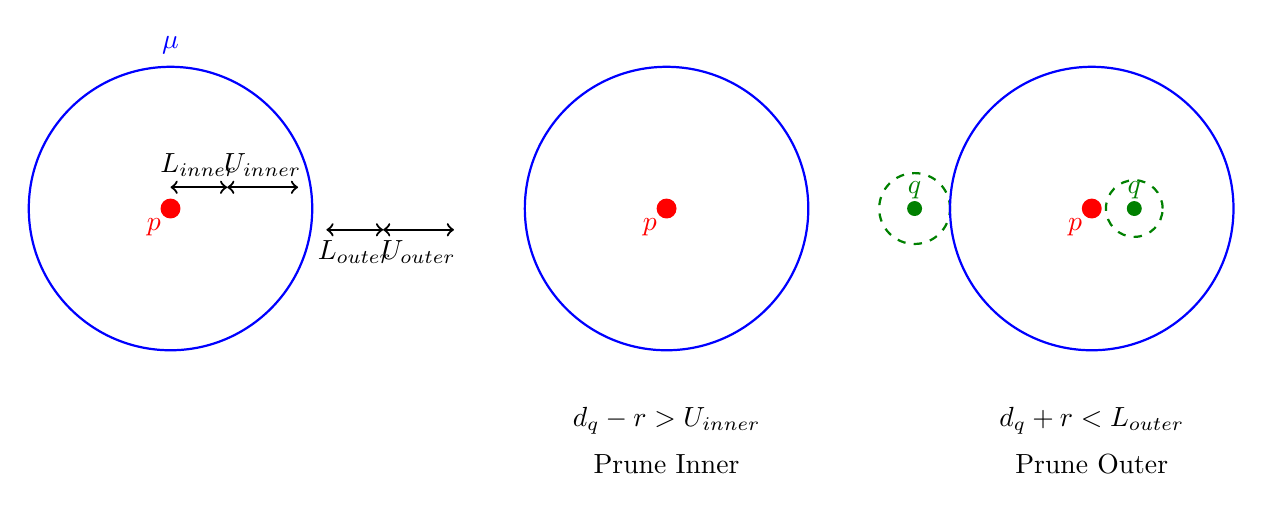
\begin{tikzpicture}[scale=0.9]
        % 左图:距离范围示意
        \fill[red] (0,0) circle (4pt) node[below left] {$p$};
        \draw[thick,blue] (0,0) circle (2);
        \node[blue] at (0,2.3) {$\mu$};

        % 沿正x方向标注距离范围(更直观)
        \draw[<->,thick] (0,0.3) -- (0.8,0.3) node[midway,above] {$L_{inner}$};
        \draw[<->,thick] (0.8,0.3) -- (1.8,0.3) node[midway,above] {$U_{inner}$};
        \draw[<->,thick] (2.2,-0.3) -- (3,-0.3) node[midway,below] {$L_{outer}$};
        \draw[<->,thick] (3,-0.3) -- (4,-0.3) node[midway,below] {$U_{outer}$};

        % 中图:Prune Inner 场景
        \begin{scope}[xshift=7cm]
            \fill[red] (0,0) circle (4pt) node[below left] {$p$};
            \draw[thick,blue] (0,0) circle (2);
            \fill[green!50!black] (3.5,0) circle (3pt) node[above] {$q$};
            \draw[thick,green!50!black,dashed] (3.5,0) circle (0.5);
            \node at (0,-3) {$d_q - r > U_{inner}$};
            \node at (0,-3.6) {Prune Inner};
        \end{scope}

        % 右图:Prune Outer 场景
        \begin{scope}[xshift=13cm]
            \fill[red] (0,0) circle (4pt) node[below left] {$p$};
            \draw[thick,blue] (0,0) circle (2);
            \fill[green!50!black] (0.6,0) circle (3pt) node[above] {$q$};
            \draw[thick,green!50!black,dashed] (0.6,0) circle (0.4);
            \node at (0,-3) {$d_q + r < L_{outer}$};
            \node at (0,-3.6) {Prune Outer};
        \end{scope}
    \end{tikzpicture}
    \caption{VP树剪枝规则示意}
    \label{fig:vp-pruning}
\end{figure}

\subsection{GHT与VPT的理论对比}

\subsubsection{数据划分方式对比}

表\ref{tab:partition-compare}对比了GH树和VP树的划分方式。

\begin{table}[htbp]
    \centering
    \caption{GH树与VP树数据划分方式对比}
    \label{tab:partition-compare}
    \begin{tabular}{lcc}
        \toprule
        \textbf{特性} & \textbf{GH树} & \textbf{VP树} \\
        \midrule
        划分方式 & 超平面划分 & 球形划分 \\
        几何形状 & 两点等距平面 & 同心球 \\
        划分平衡性 & 依赖数据分布 & 中位数保证平衡 \\
        \bottomrule
    \end{tabular}
\end{table}

\subsubsection{支撑点使用对比}

表\ref{tab:pivot-compare}对比了两种树的支撑点使用情况。

\begin{table}[htbp]
    \centering
    \caption{支撑点使用对比}
    \label{tab:pivot-compare}
    \begin{tabular}{lcc}
        \toprule
        \textbf{特性} & \textbf{GH树} & \textbf{VP树} \\
        \midrule
        每节点pivot数 & 2 & 1 \\
        pivot作用 & 定义超平面 & 定义球心 \\
        距离计算(每节点) & 2次 & 1次 \\
        剪枝信息 & 两距离差值 & 距离范围 \\
        \bottomrule
    \end{tabular}
\end{table}

\subsubsection{空间划分特性对比}

\textbf{GH树的特点}:
\begin{itemize}
    \item 优势:划分更对称,在低维空间效果好
    \item 劣势:需要2个pivot,构建开销略大
\end{itemize}

\textbf{VP树的特点}:
\begin{itemize}
    \item 优势:只需1个pivot,距离范围提供精确剪枝
    \item 劣势:球形划分可能导致空间浪费,高维情况受维度灾难影响
\end{itemize}

